
% ════════════════════════════════════════════
% 模型准备（5.4.2.模型准备.tex，三级子块）
% ════════════════════════════════════════════
\subsubsection{模型准备}

\textbf{1.数据预处理}

附件四提供了 2025 年全年每天不同时刻的外网实时波动电价，时间分辨率为 10 分钟。设第 $d$ 天第 $k$ 个间隔的波动电价为 $p_{d,k}$，则全年电价数据可组织为：
\begin{equation}
    \boldsymbol{P}=[p_{d,k}]_{365\times 144}
\end{equation}
对其进行数值化检查，全年无缺失值，电价分布范围约为 $0.3\sim 1.6$ 元/kWh。波动电价与固定电价的典型日对比如图\ref{fig:preprocess4}所示。

\begin{figure}[H]
    \centering
    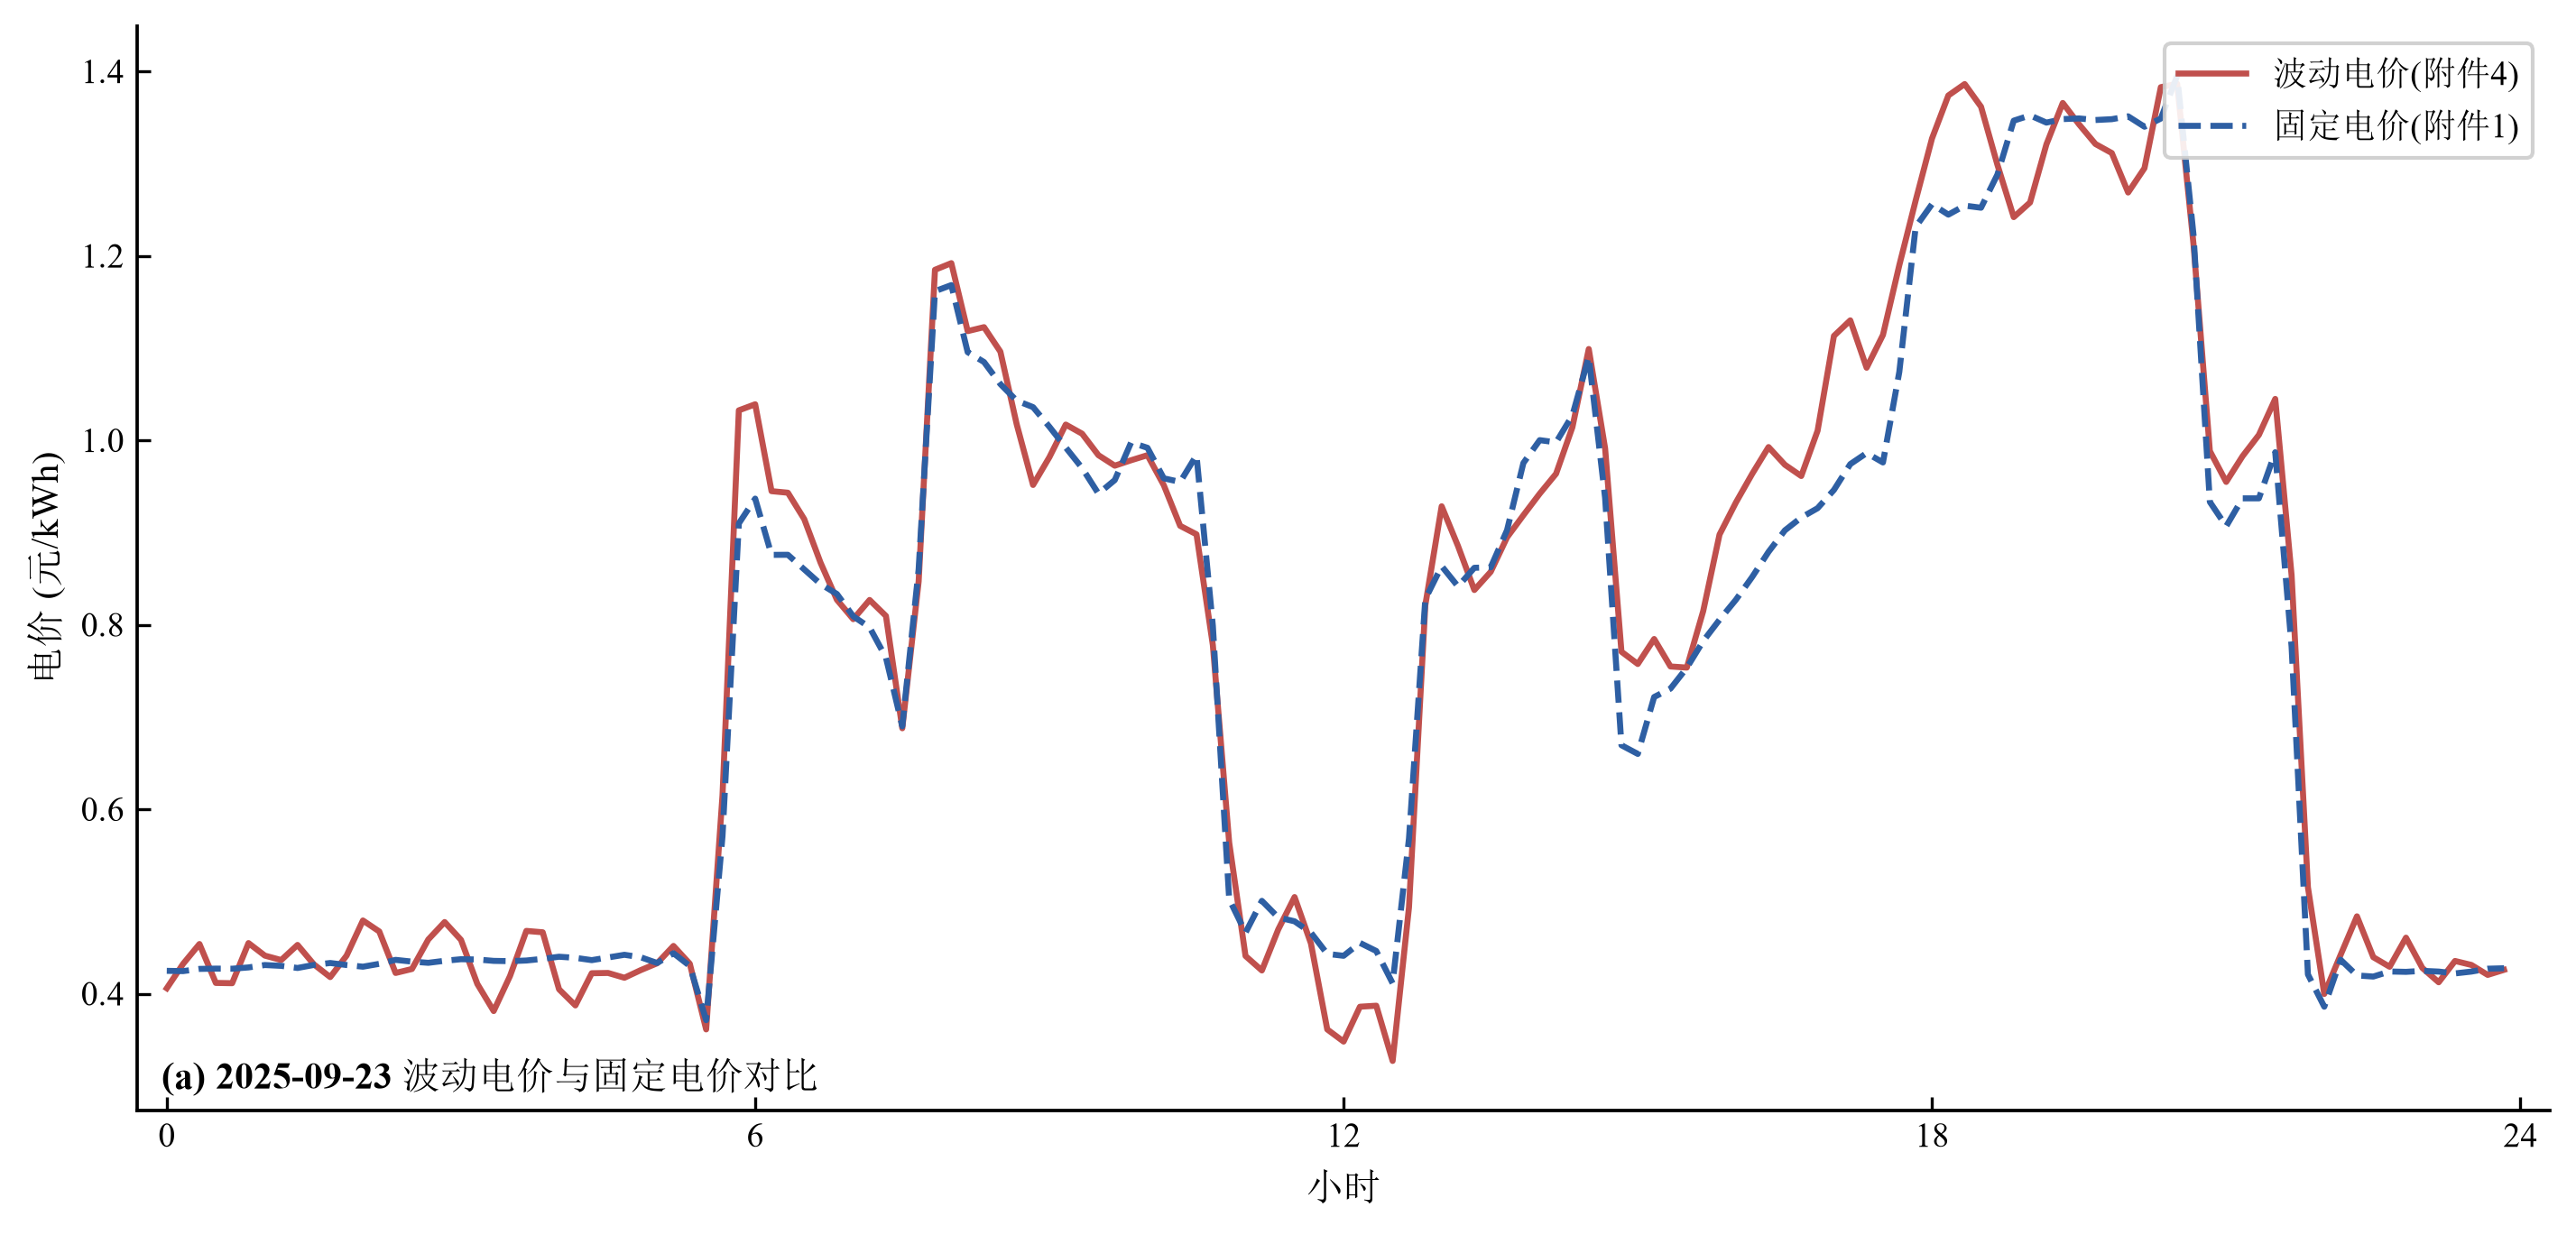
\includegraphics[width=0.70\textwidth]{求解/问题四/图片/图4-1_波动与固定电价对比.png}
    \caption{波动电价与固定电价的典型日对比}
    \label{fig:preprocess4}
\end{figure}

由图\ref{fig:preprocess4}可知，波动电价在同一天内剧烈起伏，白天用电高峰电价可达 1.5 元/kWh 以上，夜间低谷可低至 0.35 元/kWh 左右，其峰谷价差明显大于固定电价，因此储能低充高放的套利空间更大，但购电时机的把握也更为关键。

\textbf{2.算法选择}

在完成电价数据预处理后，本问的建模框架与问题二、问题三完全一致，仅将电价参数由固定序列替换为逐间隔波动序列。由于目标函数与约束仍是线性的，问题二对应部分可继续采用逐日线性规划，问题三对应部分可继续采用滚动线性规划，算法选择与前述问题一致，此处不再重复对比，仅对参数替换作说明：将式(1)中的 $p_k$ 替换为 $p_{d,k}$ 即可得到波动电价下的模型。
